\documentclass{sig-alternate}
\usepackage{amsmath}
\usepackage[T1]{fontenc}
\usepackage{ae, aecompl}
\usepackage{color}
\usepackage{booktabs}
\usepackage{paralist}
\usepackage{graphicx}
\usepackage{amsfonts}
\usepackage{times}

\usepackage{float}
%\DeclareCaptionType{copyrightbox}
\usepackage[hyphens]{url}
\usepackage{enumerate}
\usepackage{algorithmicx}
\usepackage{algpseudocode}
\usepackage{algorithm}

\usepackage{subfig}

\newcommand{\nn}{\nonumber}
\newcommand{\set}[1]{\mathcal{#1}}        			% Set
\newcommand{\rv}[1]{\boldsymbol{#1}}    			% Random variable
\renewcommand{\vec}[1]{\boldsymbol{\mathrm{#1}}} 	% Vector or Matrix
\newcommand{\event}[1]{\langle #1 \rangle}      	% Event
\newcommand{\arthur}[1]{\textcolor{blue}{Arthur: #1}}
\newcommand{\fixit}[1]{\textcolor{red}{#1}}
\newcommand{\etal}{\emph{et~al.}}


\renewcommand{\itemize}{\compactitem}
 \renewcommand{\enumerate}{\compactenum}

\newenvironment{mymathbox}
{\par\smallskip\centering\begin{lrbox}{0}%
\begin{minipage}[c]{0.8\textwidth}}
{\end{minipage}\end{lrbox}%
\framebox[0.9\textwidth]{\usebox{0}}%
\par\medskip
\ignorespacesafterend}
\begin{document}

%\title{Bitcoin Fraud with Targeted Blockchain Forks}
\title{Quantifying Web Adblocker Privacy}
%\title{Bitcoin Block and Transaction Withholding}
%\title{On Withholding Blocks and Transactions in Bitcoin}
%\title{Consequences of Withholding Blocks and Transactions in Bitcoin}
%\title{Consequences of Data Delivery Delay in Bitcoin}
%\title{Data Delivery Delay in Bitcoin}
%\numberofauthors{1}
\author{}
%\numberofauthors{1}
%\author{Arthur Gervais$^\dag$, Hubert Ritzdorf$^\dag$, Ghassan O. Karame$^\dag$, Srdjan Capkun$^\dag$\\ \medskip \affaddr{$^\dag$ETH Zurich, Switzerland} \\ \email{$^\dag$firstname.lastname@inf.ethz.ch} }

\numberofauthors{1}
%\author{$^\dag$, $^\dag$, $^\ddag$ and $^\dag$\\ \medskip \affaddr{$^\dag$ETH Zurich, Switzerland \\ \email{$^\dag$firstname.lastname@inf.ethz.ch }

\maketitle

\begin{abstract}
\end{abstract}

\section{Introduction} \label{sec:introduction}

Advertising company models: direct buy, ad networks, ad exchanges.

\begin{itemize}
\item Adblocker - browser plugin blocking web advertisements
\end{itemize}


\section{Background} \label{sec:background}
The literature employed the number of blacklisted domains as a privacy indication~\cite{XX}, but we argue that this is not a sufficient indicator for the offered privacy enhancements. Instead of only capturing the reduction in percentage of accessed third parties, we argue that the graph of third parties should be analyzed in its entirety. Certain third parties are furthermore clearly collaborating, since they belong to the same logical entity. We therefore define the following privacy metrics in order to objectively compare different adblocker.

\section{Privacy metrics} \label{sec:privacy_metrics}
In this Section we introduce the privacy metrics used in order to quantify the privacy provisions of adblocker.

%{\color{blue}We model the tracking of a user $U$ through third parties as undirected graph $G=(E,V)$, where $E$ are edges, and $V$ vertices. A vertice can represent either a first party \emph{fp} (i.e. the URL the user visits) or a third party \emph{tp} (i.e. the URL of a resource that a first party fetches). An edge is built between a \emph{fp} that fetches a \emph{tp}. By visiting a series of websites $S_U = \{w_1, w_2, .. , w_n\}$, the complete tracking graph $G$ becomes apparent.}

We model the tracking of a user $U$ through third parties as undirected graph $G=(E,V)$, where $E$ are edges, and $V$ vertices. A vertex $V_S$ represents a domain and is connected to another vertex $V_T$ through an edge $E$, if and only if at least one request has been sent from $V_S$ to $V_T$. In that case, $V_S$ is the \textit{source} of the request and $V_T$ the \textit{target} of the request.

In the following, we will use the term \textit{third-party request} (TPR) to denote the requests that are sent to a target domain that differs from the source domain and corresponds to a graph edge, $E$. On the contrary, the requests whose source and target coincide will be designated as \textit{first-party requests} (FPR) and will not be taken into consideration for the construction of $G$. The source and the target domain will be referred to as \textit{first-party domain} (FPD) and \textit{third-party domain} (TPD) and will correspond to FPD and TPD graph nodes, respectively.

We augment \emph{G} by incorporating the logical relationship between third party domains. Two \emph{tp}, belonging to the same logical entity are thus combined into one vertice, resulting in a hierarchical graph. Figure~\ref{fig:graph} visualizes the different components of the build graph. Given \emph{G}, we evaluate the respective privacy provisions based on the following metrics.

\begin{figure}[htb!]
  \centering
  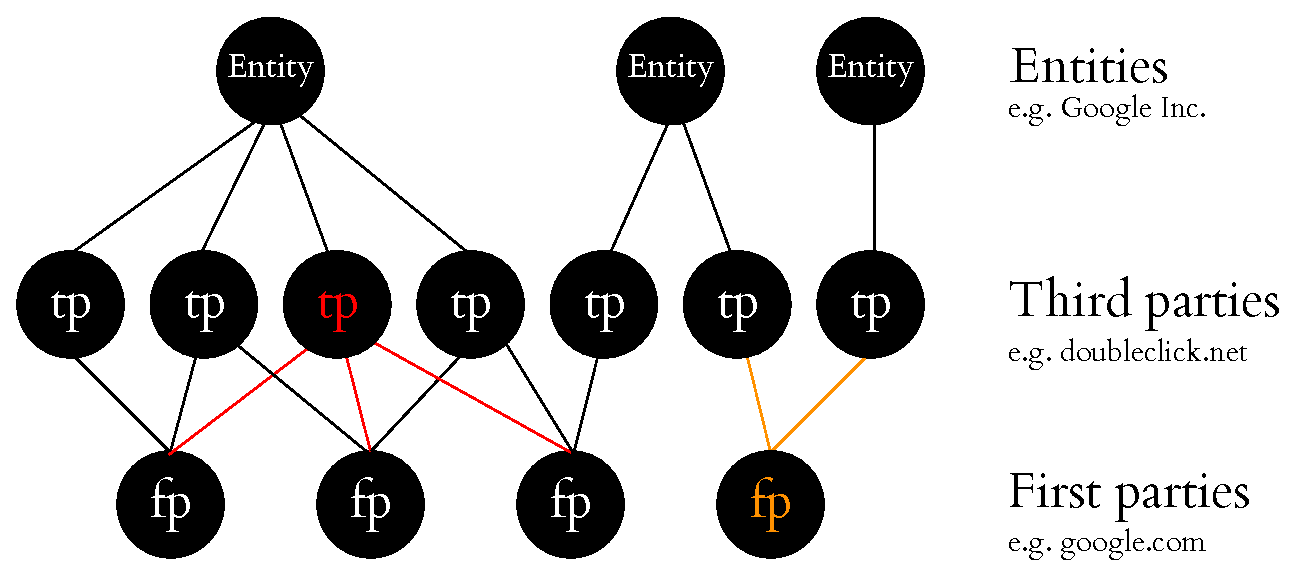
\includegraphics[width=0.45\textwidth]{figures/graph.eps}
  \caption{Graph built based on the regular crawling of the respective first parties. The colored third party has a node degree of 3, the colored first party has a node degree of 2.}\label{fig:graph}
\end{figure}

\paragraph{Add metric of how the BL changes (+ or - entries)}
\paragraph{Randomness of advertisement?}

\paragraph{Degree of first party}
The more third parties a first party loads, the more likely the user is tracked. We therefore assess the number of edges of the first parties, equivalent to the degree of the first party vertices in graph $G$. By comparing the reduction in first parties with and without adblocker, we can objectively compare the improvement in the offered privacy of an adblocker.

\paragraph{Degree of third party}
The more often a third party is accessed over the users' series of websites $S_U$, the less privacy the user experiences from this particular third party. This intuition can be explained as follows. Let's assume that a third party is only loaded once from a first party in the series of websites $S_U$ loaded by $U$. This third party will learn that the user has accessed the respective first party, but has a limited view of the surf behavior of $U$. If the third party, however, is requested in over 80\% of the users' visited websites, the third party is likely to recover 80\% of the users' web behavior.

We capture this privacy notion, by assessing the degree of the third party nodes in the graph $G$ with respect to first parties.
Similar to the degree of first parties, we can then evaluate the improvement in the offered privacy of an adblock software.

\paragraph{Graph density}
In addition the the outlined privacy metrics, we consider the graph density of $G$. The more dense $G$ is, the more third parties are likely to be able to track the user $U$. The graph density therefore allows to reason about the possible privacy improvements by the respective adblock software. For undirected graphs, the graph density is commonly defined as:
\begin{equation}
D = \frac{2 |E|}{|V|(|V|-1)}
\end{equation}

Note, that we cannot achieve the maximum density of 1, because the first parties are usually not directly connected.

\paragraph{Blacklist latency}
The formerly presented metrics only allow us to reason about the privacy provisions of the advertisement blocking software at a given time $t$. The advertisement industry, however, operates dynamically by using e.g., new advertisement techniques and new third party URLs. In order to capture the temporal privacy provisions of the adblocker, we evaluate the the aforementioned privacy metrics over a timespan of several months. This allows us to reason quantitatively about how fast an adblocker adapts to a changing advertisement environment.

\subsection{Beyond URLs}
The presented metrics capture the raw third party URLs. Since the URL information, however, does not capture many aspects of the respective web infrastructure and resulting privacy risks, we augment the graph $G$, by incorporating, logical entities, cookies, and if a third party contains active or passive content.

\paragraph{Logical entity}
Instead of focusing on the URL of a third party, we link the third parties based on their respective owner information. Third parties such as \url{doubleclick.net} and \url{google.com} for example are both owned by the same entity Google Inc. Their collusion therefore seems more likely, and affects the privacy of a web user $U$ more significantly, than if both were belonging to two different logical entities. By incorporating the logical relation among third party domains, we therefore capture a more realistic privacy leakage through user web surf activity.

\paragraph{DNT influence}
Does DNT change something (has been studied before).

\section{Evaluation}

\subsection{Experimental setup}

\subsubsection{Lightbeam first-partyness heuristics}
{\color{blue}probably mention that it is not a mistake but it only is not in accordance with what WE define as first and third party}
The distinction between FPRs and TPRs is crucial in our attempt to precisely quantify the ad-blocking efficiency for each user profile $U$, since they define the exact topology of the derived graph $G$. Although Lightbeam already implements an algorithm to decide over the ``first-partyness'' of a request, so as to create this graph, it does not have the exact knowledge of the actual website visited. To compensate for this lack of information, Lightbeam applies a few heuristics in order to estimate which source domain initiated the request, compares it to the already-known target domain of the request and followingly classifies it as a FPR or TPR.

By examining the request logs after a complete crawl cycle and comparing the estimated source to the actual crawled domain, two types of false-positive cases (Table \ref{table:false_positive_examples}) arise:

\begin{itemize}
\item \textbf{Unrecognized TPRs:} The request is mistakenly considered to be a FPR according to the Lightbeam heuristics, this way ``hiding'' a TPR edge from the graph.
\item \textbf{Misclassified TPRs:} The request is correctly found to be a TPR, but not for the correct FPD node, i.e. the one corresponding to the actually crawled domain. The inaccuracy introduced to the graph results from the potential introduction of a bogus FPD node, as well as the false number of TPR edges starting from the correct and the bogus FPD nodes.
\end{itemize}

{\color{red}what is the exact value? For how many first parties did we check this. What is the error of unrecognized TPRs, what is the error of misclassified TPRs?}
{\color{blue}
As results from the experimental evaluation on the data of one full crawl cycle (1000 visited first parties) and 12 different user profiles, the misclassified and unrecognized TPRs make up for 2.0\%-12.0\% and 4.0\%-11.0\% of the total requests, accordingly. The percentages differ for the various user profiles examined.}

\begin{table}
\centering
\small
\begin{tabular}{|c|c c c|}
\hline
& Visited Domain & Estimated Source & Target \\
\hline
Recognized & wp.pl & wp.pl & facebook.com \\
Misclassified & wp.pl & facebook.com & fbcdn.net \\
Unrecognized & wp.pl & facebook.com & facebook.com \\
\hline
\end{tabular}
\caption{Examples of misclassified and unrecognized TPRs}
\label{table:false_positive_examples}
\end{table}

\subsubsection{Our crawler}
\paragraph{User profiles}
\label{sec:user_profiles}
In order to compare the efficacy of different adblockers, as well as the influence of different browser settings on their adblocking efficiency, we create 12 user profiles, $U$, each of which will be defined as a combination of the following parameters (Table \ref{table:user_profiles}){\color{red}Please make a table with all the profiles}:

\begin{itemize}
 \item Ad-blocker installed
 \item Block policy: The blacklists applied or the list of blocked trackers is set to its default state or set so as to provide a maximal protection
 \item Mobile or Desktop User Agent
 \item Do Not Track (DNT) header enabled
\end{itemize}


\paragraph{Crawled URLs}
{\color{red}Please describe how our crawler works.}
{\color{blue}
An appropriate criterion for the evaluation of an adblocker is its performance in the most frequent case. Consequently, it would be plausible to test its efficiency for the \textit{500 domains with the highest incoming web traffic}. Nonetheless, considering only the top-visited domains in our evaluation would imply the risk of favoring an adblocker optimized to perform better for a certain group of websites, eventually biasing our experimental results. An appropriate countermeasure would hence be to extend our URL sample set with another \textit{500 randomly chosen domains} among the top 1 million most-visited domains. The sample set $W$ of 1000 URLs is extracted using the Alexa Traffic Rank as a reference point and is stored and kept unchanged throughout the whole evaluation period, so as to decorrelate any variations of the results between two different days from the selection of the sample set $W$.

Since nowadays most of the web applications are based on asynchronous calls to fetch data, when the DOM has finished rendering, only a part of the content has been downloaded in most of the cases, or equivalently, not all of the requests have been sent to any first or third parties to fully load the page content. Therefore, to collect the complete data and better simulate the common user browsing behavior, the crawler will wait 20 seconds on each website of our sample set $W$ and record any requests sent, before closing it and proceeding to the next domain. Additionally, to achieve independency from any heuristics in our attempt to determine the source of a request, we augment the request data provided by \textit{Lightbeam} with the actual knowledge of the currently visited first-party.

Last but not least, in order to decouple the experiment conditions from the influence of any time- or location-related effects --i.e. variations of the served content, locale-based personalization-- all user profiles $U$ will execute the same crawling routine simultaneously, whilst running on the same machine, thus behind the same IP address.
}

\subsection{Experimental Results}
{\color{blue} For a more effective overview of the experimental results for each user profile $U$, the following conventions are used in the graphs:
\begin{itemize}
 \item The \textit{color} denotes the adblocker installed.
 \item The \textit{line width} indicates the protection degree --i.e. default settings as opposed to the maximal protection achieved through the use of maximum block policy or the DNT header.
 \item Profiles with mobile agent are plotted in \textit{dashed lines}.
\end{itemize}
The plot legends for each user profile $U$ are listed in more detail in Table \ref{table:user_profiles}.
}

\afterpage{

  \begin{table}
  % Defining dash lines
  \newcommand\solidthinrule[1][.5cm]{\rule[0.5ex]{#1}{.4pt}}
  \newcommand\solidthickrule[1][.5cm]{\rule[0.5ex]{#1}{1.5pt}}
  \newcommand\dashedthinrule{\mbox{%
    \solidthinrule[1mm]\hspace{1mm}\solidthinrule[1mm]\hspace{1mm}\solidthinrule[1mm]}}
  \newcommand\dashedthickrule{\mbox{%
    \solidthickrule[1mm]\hspace{1mm}\solidthickrule[1mm]\hspace{1mm}\solidthickrule[1mm]}}
  \definecolor{darkgreen}{rgb}{0, 0.8, 0}
    
  \centering
  \tiny
  \begin{tabular}{|c|c c c c c|}
  \hline
  User Profile & Adblocker & Block Policy & DNT & User Agent & Legend \\
  \hline
  Ghostery\_Default & Ghostery & Default & No & Desktop  & {\color{red}\solidthinrule} \\
  Ghostery\_MaxProtection & Ghostery & Max & No & Desktop & {\color{red}\solidthickrule} \\
  Adblockplus\_Default & AdblockPlus & Default & No & Desktop & {\color{blue}\solidthinrule} \\
  Adblockplus\_MaxProtection & AdblockPlus & Max & No & Desktop & {\color{blue}\solidthickrule} \\
  NoAdblocker & None & - & No & Desktop & {\color{red}\solidthinrule} \\
  NoAdblocker\_DNT & None & - & Yes & Desktop & {\color{darkgreen}\solidthickrule} \\
  Ghostery\_Default\_MUA & Ghostery & Default & No & Mobile & {\color{darkgreen}\dashedthinrule} \\
  Ghostery\_MaxProtection\_MUA & Ghostery & Max & No & Mobile & {\color{red}\dashedthickrule} \\
  Adblockplus\_Default\_MUA & AdblockPlus & Default & No & Mobile & {\color{blue}\dashedthinrule} \\
  Adblockplus\_MaxProtection\_MUA & AdblockPlus & Max & No & Mobile & {\color{blue}\dashedthickrule} \\
  NoAdblocker\_MUA & None & - & No & Mobile & {\color{darkgreen}\dashedthinrule} \\
  NoAdblocker\_DNT\_MUA & None & - & Yes & Mobile & {\color{darkgreen}\dashedthickrule} \\
  \hline
  \end{tabular}
  \caption{Overview of user profiles examined}
  \label{table:user_profiles}
  \end{table}

  \begin{figure}
   \centering
   
   \subfigure{
    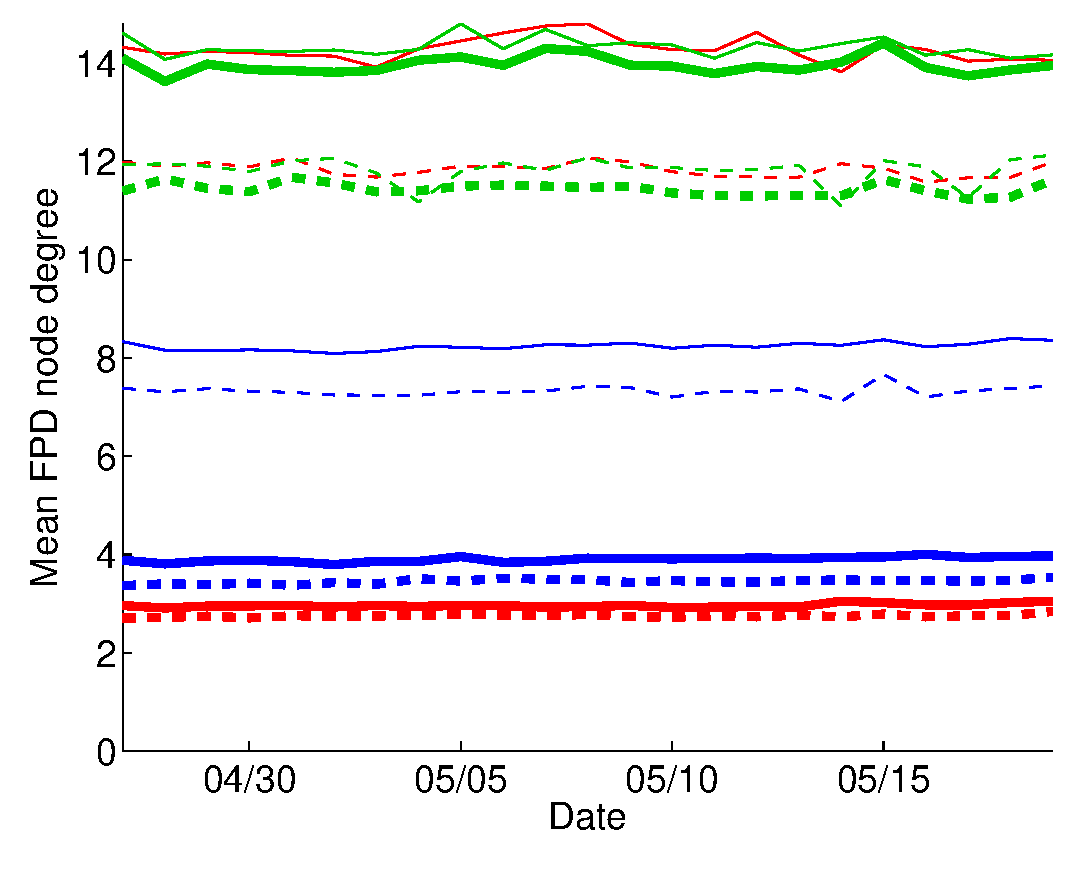
\includegraphics[width=0.45\textwidth]{figures/plots/first-means.eps}
    \caption{Mean value of the degree of the first-party nodes, $V_S$ over time for each user profile $U$}
    \label{fig:first_means}
  }
  \subfigure{
    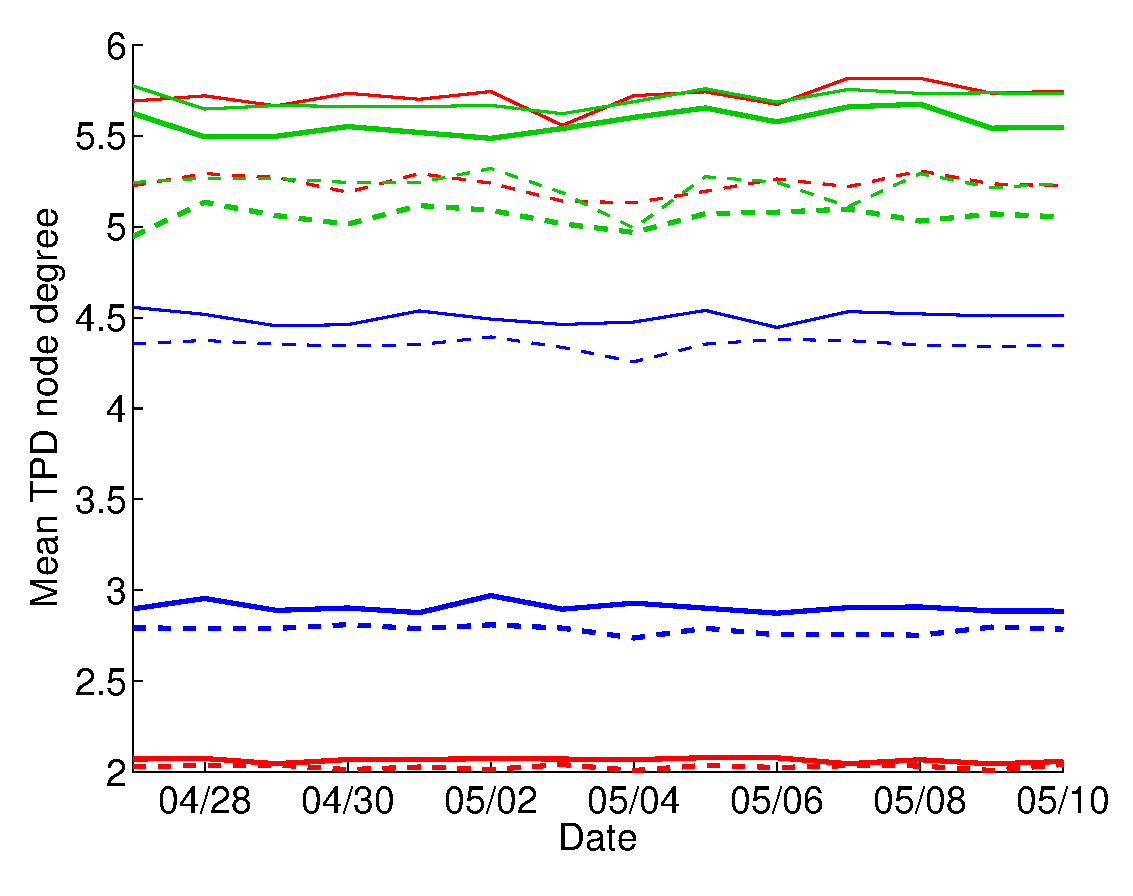
\includegraphics[width=0.45\textwidth]{figures/plots/third-means.eps}
    \caption{Mean value of the degree of the third-party nodes, $V_T$ over time for each user profile $U$}
    \label{fig:third_means}
  }

  \subfigure{
    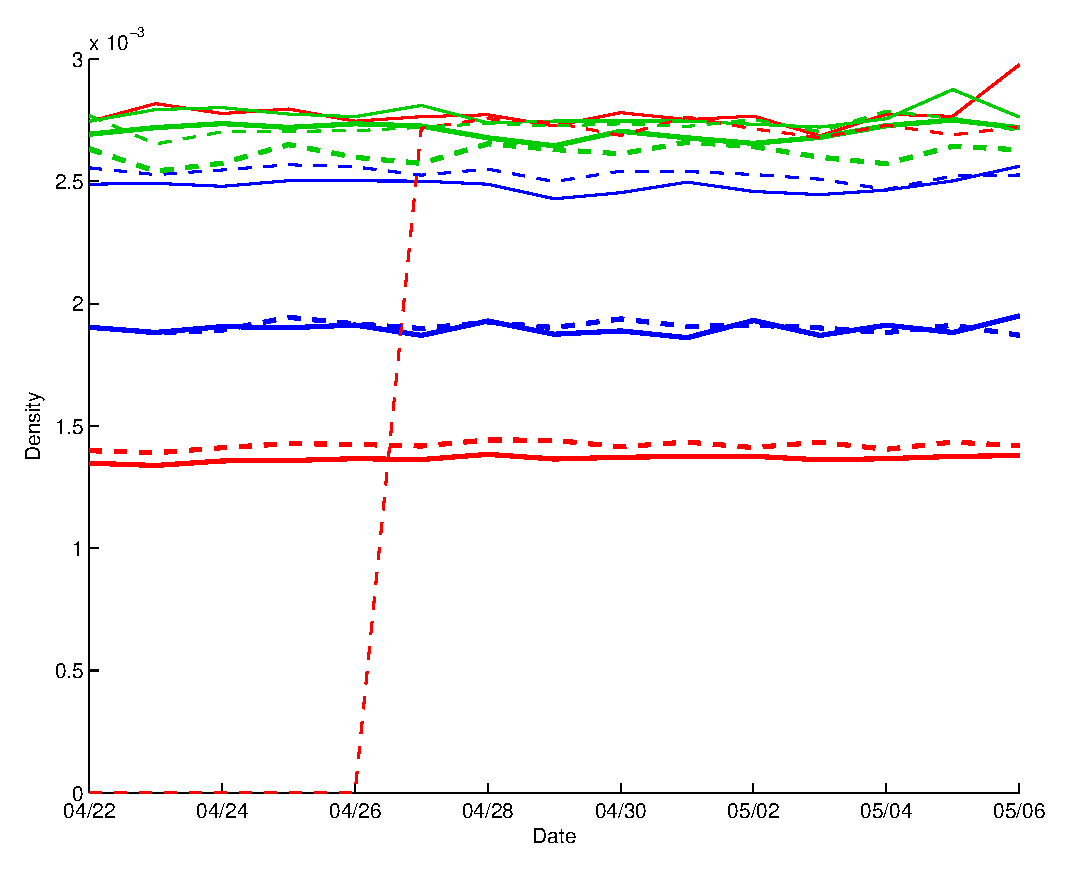
\includegraphics[width=0.45\textwidth]{figures/plots/density.eps}
    \caption{Density of graph $G$ over time for each user profile $U$}
    \label{fig:density}
  }
  \end{figure}

  
}

\subsubsection{First Party Node Degree}
{\color{blue}As depicted in Figure \ref{fig:first_means}, the user profiles \textit{Ghostery\_Default} and \textit{NoAdblocker} have the worst performance, since the first parties they visit load the highest mean number of third parties. Although we would expect that the use of an adblocker, such as Ghostery, should provide us with better results, a closer look at its initial settings show that the adblocker functions as a third-party tracker that does not block any third parties by default, unless configured appropriately. The metric has a consistently but only slightly lower value for the profile \textit{NoAdblocker\_DNT}.

A steadily better performance is to be observed for the user profiles with the exact same settings as above, but with a Mobile User Agent, i.e. \textit{Ghostery\_Default\_MUA}, \textit{NoAdblocker\_MUA} and \textit{NoAdblocker\_DNT\_MUA}, where the mean node degree is markedly lower and the relative order of the three profiles remains unaltered.

A significantly better result comes with the use of AdblockPlus, since the profiles \textit{Adblockplus\_Default} and \textit{Adblockplus\_Default\_MUA} using AdblockPlus with its default settings have a mean node degree about 40\% lower than the aforementioned worst cases. This result is particularly important, because they indicate the advantage of using an adblocker, even with minimal settings --but not disabled, as in the case of \textit{Ghostery\_Default}.

Nevertheless, the most efficient user profiles from an adblocking viewpoint are, as expected, the profiles that have not only an adblocker installed, but have also configured it to a maximal-protection level. In this case, a mean node degree up to nearly 80\% lower is achieved with respect to the default case, while to be pointed out is the fact that Ghostery performs constantly compared to AdblockPlus, when both are compared under equal terms, i.e. manual settings to achieve an optimal result.}

\subsubsection{Third Party Node Degree}
{\color{blue}An observation of the experimental results for the mean third-party node degree of the graphs $G_U$ for each user profile $U$, as plotted in Figure \ref{fig:third_means} confirms the conclusions of our analysis so far. The relative performance of the user profiles remains unaltered, with the \textit{Ghostery\_Default} and \textit{NoAdblocker} to fare worst, whilst the user profiles with Ghostery and maximal-protection settings give us the best results. However, the discrepancies between the results of the profiles are not as remarkable as before, thus making the metric less suitable when profiles with smaller efficiency differences are to be distinguished.}

\subsubsection{Graph Density}
{\color{blue}The interpretation of the graph-density results for each of the profiles under scrutiny yields, as expected, the same results, reaffirming the evaluation of the previous sections, albeit the metric presents an even poorer ability to make fine distinctions between similarly-performing user profiles.}

\subsection{Influence of profile parameters}
{\color{blue}As explained in \ref{sec:user_profiles}, the user profiles $U$ are created as a combination of different parameters that needed to be scrutinized. After a thorough examination of the experimental results of the previous sections, the influence of these parameters can be summarized as follows:

\textbf{Adblocker installed:} As experimentally confirmed, the use or no use of an adblocker is the most decisive factor when it comes to being tracked by third parties, since even with the minimal-protection settings, the mean first-party node degree can improve by up to 40\%. The profiles with Ghostery installed under default settings have to be excluded from this analysis, however, since Ghostery has its adblocker functionality initially disabled, as discussed above. Additionally, the selection of the adblocker can also play an important role, as the comparison of the Ghostery and AdblockPlus under maximal-proteciton settings indicated.

\textbf{Block policy:} The block policy configured for each adblocker is of crucial importance, as results from the considerable contrasts between the profiles with default and maximal-protection policies --an improvement of almost 80\% and 50\% was achieved in the mean first-party degree for Ghostery and AdblockPlus, respectively.

\textbf{Do Not Track header:} The reason that the influence of this parameter is not as notable as in the other cases is the fact that the browser user has no control over whether the DNT flag is honored or not and hence websites and advertisers may either obey or completely ignore it.

\textbf{Mobile User Agent:} Websites that received requests by a mobile user agent indeed responded with a considerably lower number of third parties. A plausible explanation for this behavior is the requirement for less bandwidth that the mobile websites usually conform to. As a consequence of this limitation, less content is loaded and hence less requests are sent to third parties. This discrepancy was of course less obvious for the user profiles with maximal protection enabled, since tracking by third parties is already reduced.

As far as the graph density is concerned, it is to be observed that the performance worsens with the use of a Mobile User Agent. The reason behind this behavior is that from all of the third parties that were loaded under a Desktop User Agent, only the most popular ones --i.e. the ones that have a higher chance of being requested by more first parties, such as doubleclick.net-- are still loaded under a Mobile User Agent, which leads to a more connected graph despite the lower degree of each of its nodes.
}

\subsubsection{Blacklist latency}

\subsection{Practical considerations}
\begin{itemize}
\item Network Prediction services should be disabled (e.g. Chrome offers this option.) if these requests are not captured by the adblocker.
\end{itemize}

\section{Related work}
{\color{red}Can you add all papers that we know about and describe each in 2-3 sentences? Here we can make the link with the Lightbeam mistakes.}
{\color{blue}
\textit{Pujol et al} in \cite{pujol} aim to infer the use or no use of an adblocker by examining the HTTP(S) requests sent by a browser, using the ratio of the ad requests and the downloads of filter lists as indicators. Moreover, the performance of 7 different user profiles --adblocker-configuration combinations-- is compared based upon the total number of unblocked requests per user profile. Futhermore, the ad traffic is examined through the analysis of the number of requests at different time instances throught the day, the content-type of the ad requests, as well as the effect of enabling non-intrusive ads.
\textit{Ruffell et al} in \cite{ruffel2015} analyze the effectiveness of various browser add-ons in mitigating and protecting users from third-party tracking networks. In total 7 user profiles are created, each with a different combination of multiple add-ons and browser settings, and each of the profiles visits the 500 top Alexa Rank websites, while the HTTP request data is recorded with the use of Mozilla Lightbeam. The data is collected for one crawling cycle and followingly the efficiency analysis is performed based upon various graph metrics. ??probably subject to time variations, because experiments (user profiles) are examined serially and not in parallel (III.A)??
\textit{Mayer and Mitchell} implemented in \cite{mayer} the tool FourthParty --an open-source platform for measuring dynamic web content-- as an extension to Mozilla Firefox. Afterwards, they created several user profiles, so as to test the efficiency of different adblocking tools under certain settings (blacklists) and crawled the 500 top Alexa websites three times using FourthParty, in order to extract the average decrease in tracking with the use of the ad-blocking tools.
}

NSDI 2013 Google, alexis
https://cyberlaw.stanford.edu/files/publication/files/trackingsurvey12.pdf
Advertisement bidding
ublock.org is a lightweight blocking proxy
https://trackography.org/

\section{Conclusions} \label{sec:conclusions}

\bibliographystyle{plain}
\bibliography{relatedwork}
\end{document}
